% Created 2022-05-24 Tue 22:44
% Intended LaTeX compiler: pdflatex
\documentclass[t,10pt,xcolor={dvipsnames}]{beamer}
\usepackage[utf8]{inputenc}
\usepackage[T1]{fontenc}
\usepackage{graphicx}
\usepackage{grffile}
\usepackage{longtable}
\usepackage{wrapfig}
\usepackage{rotating}
\usepackage[normalem]{ulem}
\usepackage{amsmath}
\usepackage{textcomp}
\usepackage{amssymb}
\usepackage{capt-of}
\usepackage{hyperref}
\AtBeginSection[]{\begin{frame}<beamer>\frametitle{}\tableofcontents[currentsection]\end{frame}}
\definecolor{Orange}{rgb}{1,0.5,0}
\usepackage{listings}
\usetheme{Madrid}
\author{Mark Tullsen, William Harris, Peter Wyatt}
\date{\today}
\title{Strengthening Weak Links in the PDF Trust Chain}
\hypersetup{
 pdfauthor={Mark Tullsen, William Harris, Peter Wyatt},
 pdftitle={Strengthening Weak Links in the PDF Trust Chain},
 pdfkeywords={},
 pdfsubject={},
 pdfcreator={Emacs 27.2 (Org mode 9.4.4)}, 
 pdflang={English}}
\begin{document}

\maketitle
\begin{frame}{Outline}
\tableofcontents
\end{frame}

\section{Pre-DOM: "What Lies Beneath" is a Concern}
\label{sec:orgde9a251}
\begin{frame}[label={sec:orgb63bfd2}]{PDF Complexity?}
\begin{center}
 { \hspace{5pt}
   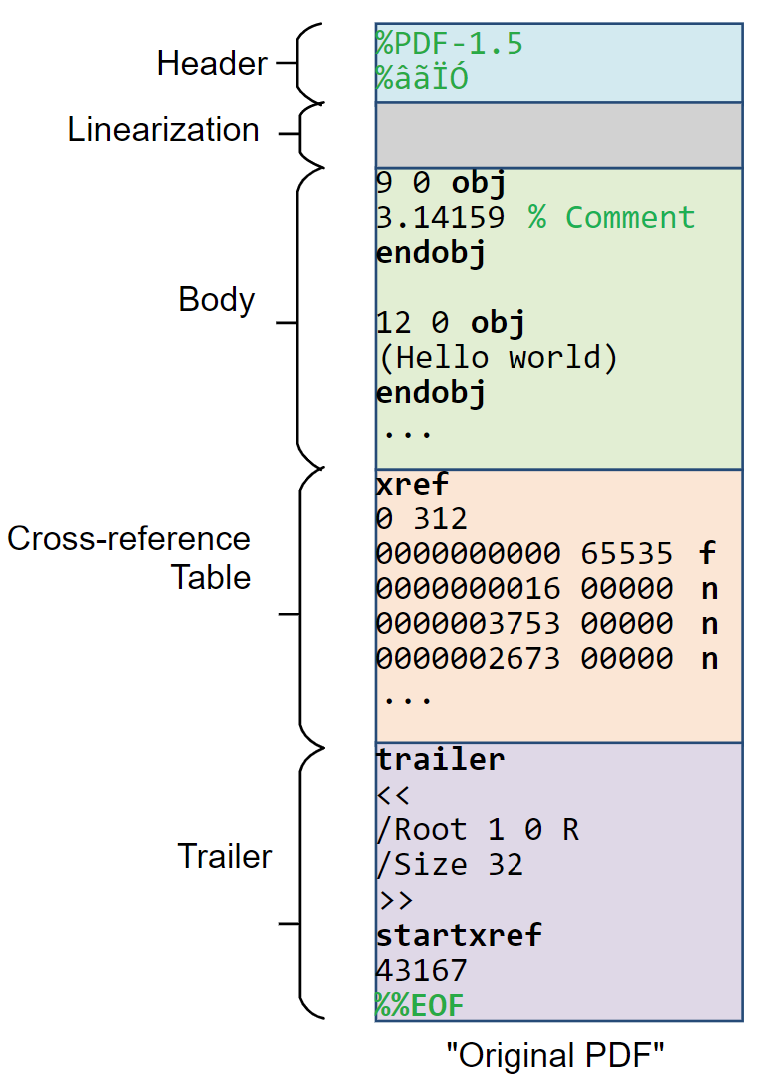
\includegraphics[width=0.4\linewidth]{../figures/pdf-structure.png}
 } \hspace{30pt}
 \raisebox{-1\baselineskip}
          {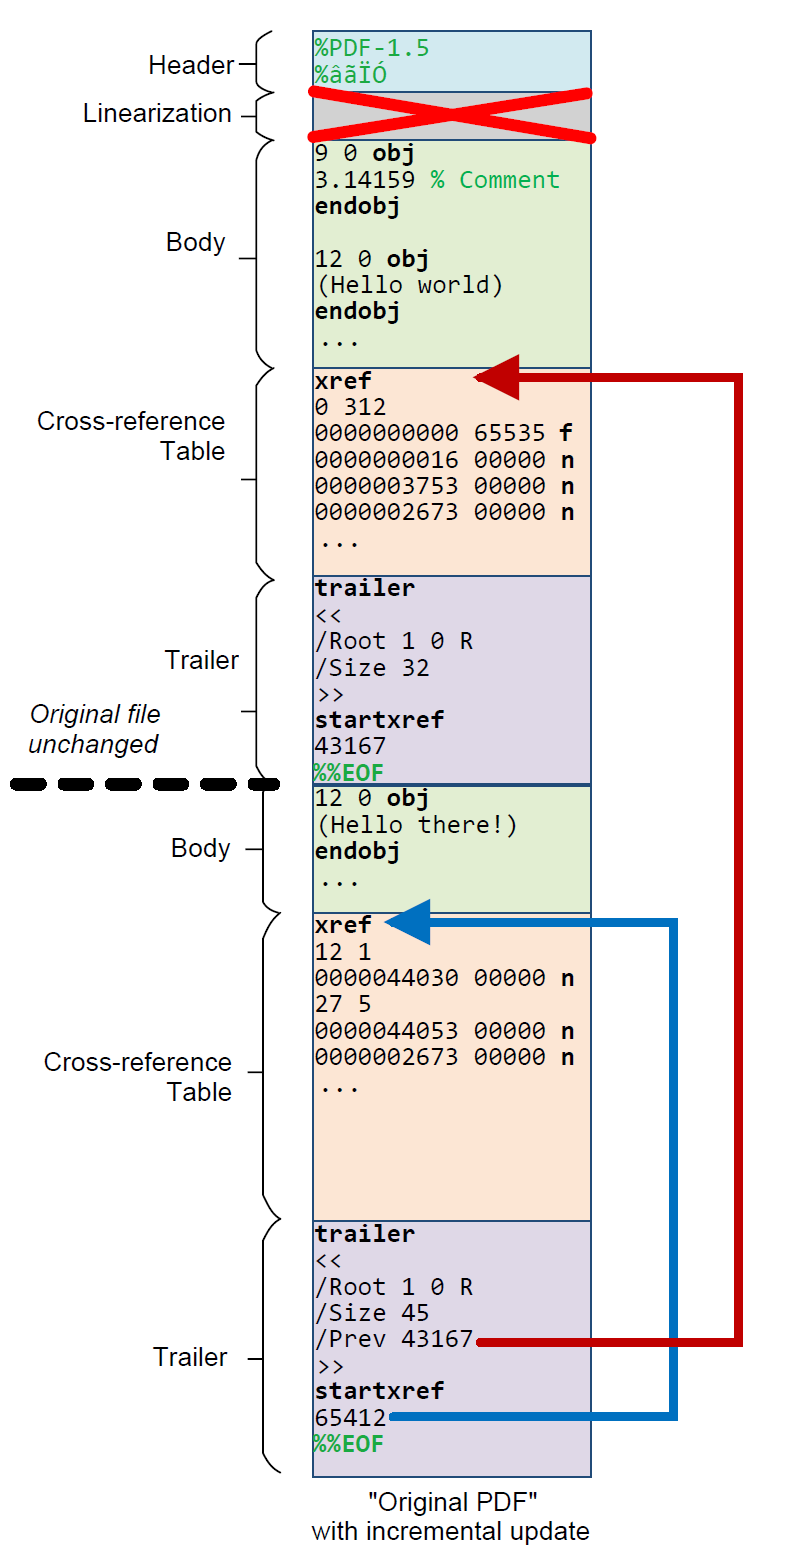
\includegraphics[width=0.30\linewidth]{../figures/pdf-structure-incremental.png}}
\end{center}
\end{frame}

\begin{frame}[label={sec:org3daab85}]{PDF Trust Chain}
\begin{center}
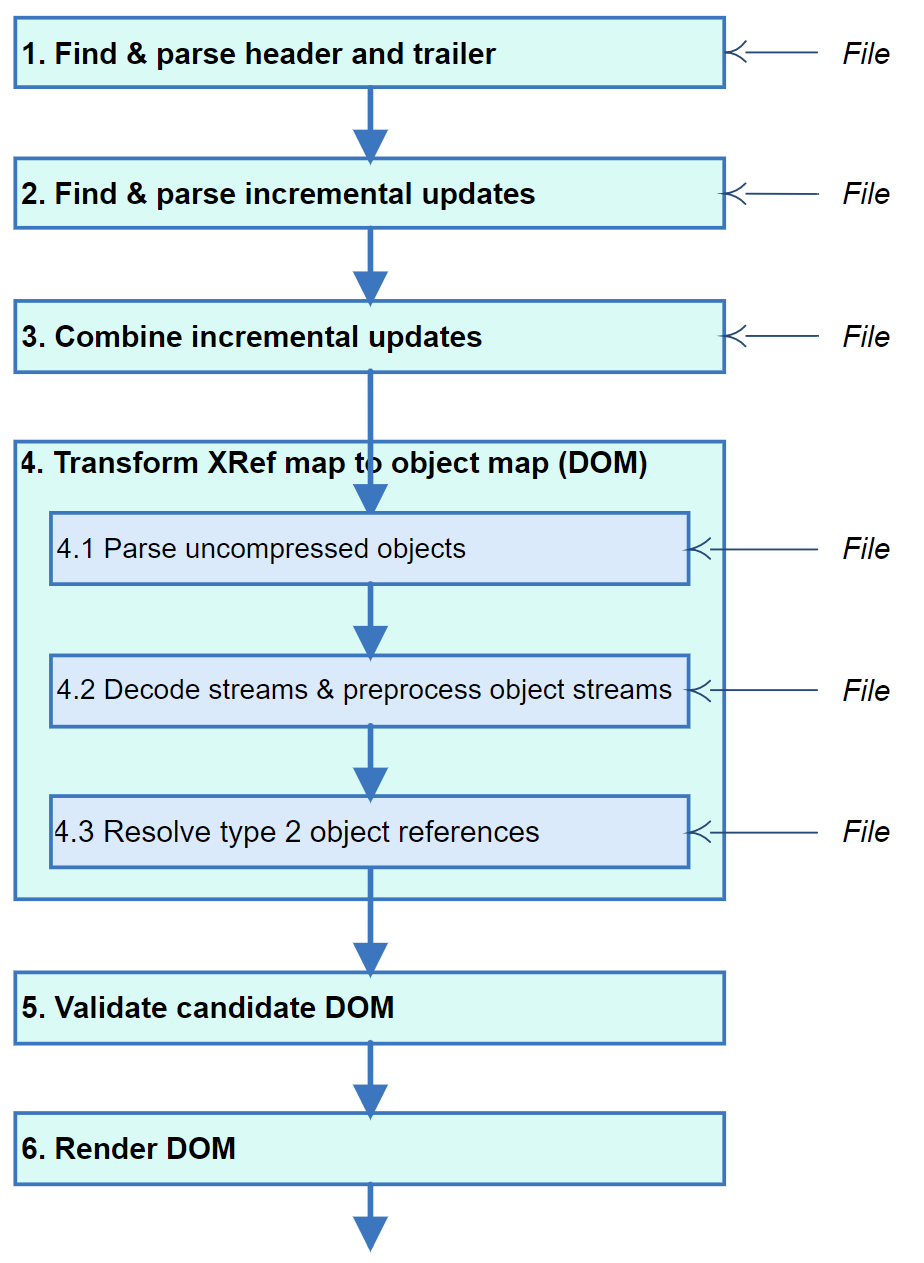
\includegraphics[width=0.47\linewidth]{../figures/Stages.png}
\end{center}
\end{frame}

\begin{frame}[label={sec:orgc8262a8}]{Vulnerabilities Occurring Primarily Pre-DOM}
\begin{itemize}
\item Schizophrenic files (different tools, different renderings)
\item Polyglot files (file being in 2+ formats)
\item Shadow attacks
\begin{itemize}
\item i.e., attacker can add "shadow content" that is PDF-signed, then reveal
at will without giving clear warnings to user.
\end{itemize}
\end{itemize}

\begin{itemize}
\item possible because of ability to sign \alert{dead objects} and \alert{cavities}
\end{itemize}
\begin{itemize}
\item Multiple places for hidden/unused/malicious data in PDF
\begin{itemize}
\item non-obvious places, unnoticed when "simply parsing"
\item e.g., shadow-attacks
\item dead bytes, dead objects, dead updates, dead linearization sections, etc.
\end{itemize}
\end{itemize}
\end{frame}

\begin{frame}[label={sec:orge1630f0}]{PDF, and Pre-DOM, Challenges}
\begin{itemize}
\item Lack of formality in standard. Thus, implementations:
\begin{itemize}
\item are more effort
\item over implement, under implement, wrongly implement
\end{itemize}
\item No definition of acceptable, reasonable error recovery
\item Less than ideal design that reflects 27 years of an evolving standard
\item Pre-DOM processing
\begin{itemize}
\item is where many parsing errors \& recovery occur
\item is non-trivial
\item involves multiple interdependent features
\item involves multiple redundant features
\begin{itemize}
\item schizophrenic if these features aren't mutually consistent
\end{itemize}
\end{itemize}
\end{itemize}
\end{frame}

\section{Modeling Pre-DOM: Highlights}
\label{sec:org6478eeb}
\begin{frame}[label={sec:org75237ea},fragile]{Stage 4: Transform XRef Map to Object Map}
 \begin{center}
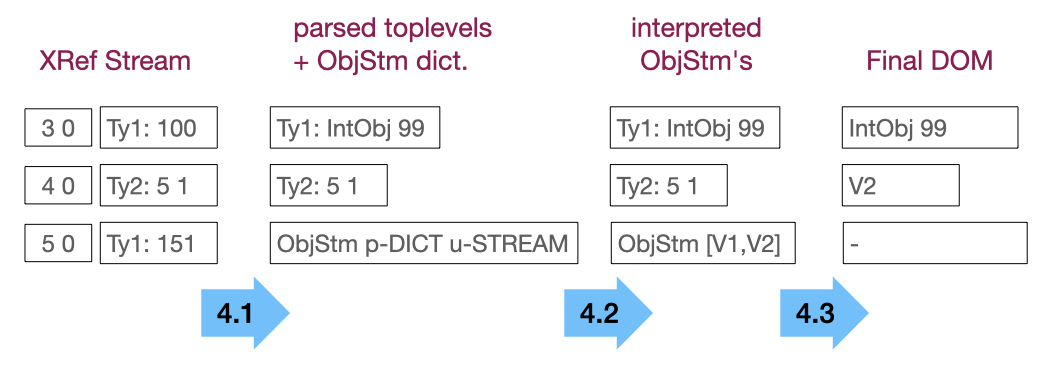
\includegraphics[width=0.8\linewidth]{images/diagram1/cropped-diagram1.001.png}
\end{center}
\lstset{language=bash,label= ,caption= ,captionpos=b,numbers=none}
\begin{lstlisting}
      ...
100   3 0 obj 99 endobj
123   % object 4 is not here
151   5 0 obj
      <<
      /Type /ObjStm
      /Length 3 0 R   % indirect!
      /N 2            % 2 objects; (potentially indirect)
      /First 10       % offset to 1st object (potentially indirect)
      >>
      stream
      4 0 6 100
      V1 % PDF-Value here, 4 0 R, [fake comment] 
      V2 % PDF-Value here, 6 0 R, [fake comment]
      endstream
      endobj
409   7 0 obj ... endobj
      ...
\end{lstlisting}
\end{frame}

\begin{frame}[label={sec:orgba88b4d}]{Parser NEQ Validator}
Validator: only valid PDFs can produce DOM (must Fail otherwise)

\vspace{10pt}
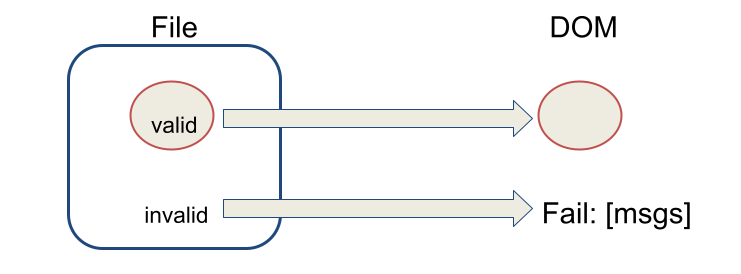
\includegraphics[width=0.90\linewidth]{images/pNEQv-1.png}
\end{frame}


\begin{frame}[label={sec:org772cdd4}]{Parser NEQ Validator}
Parser: efficiently, construct the correct DOM when a valid PDF
\vspace{10pt}
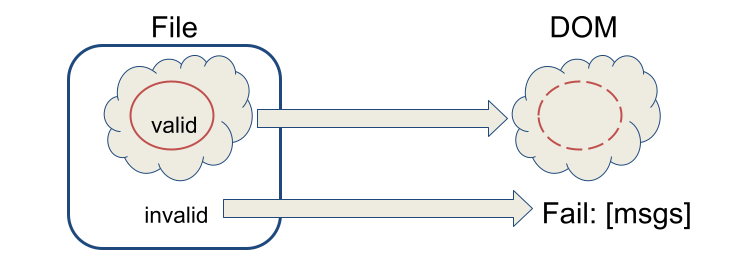
\includegraphics[width=0.90\linewidth]{images/pNEQv-2.png}
\end{frame}

\begin{frame}[label={sec:orgbc1f356}]{Parser NEQ Validator}
\vspace{20pt}
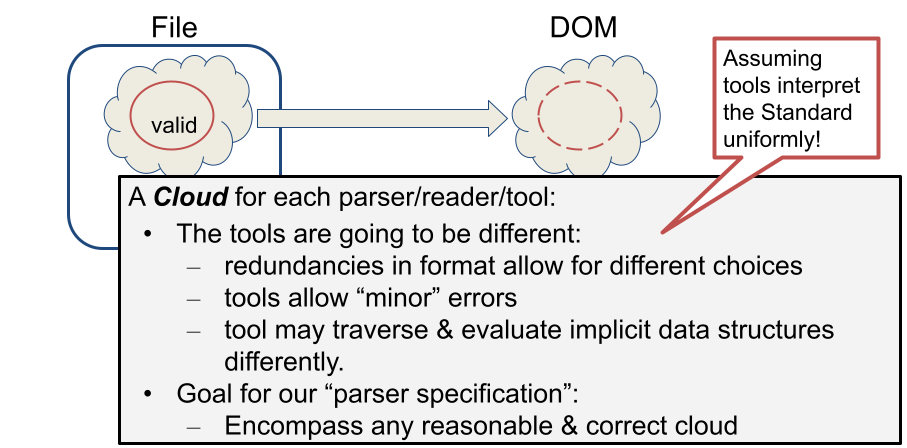
\includegraphics[width=0.90\linewidth]{images/pNEQv-3.png}
\end{frame}

\begin{frame}[label={sec:orga2eecdb},fragile]{Turning Parser into Validator}
 Parser specification is designed to be
\begin{itemize}
\item understandable: clear, pure Haskell
\item phased, clearly terminating (get parallelizability for free)
\item very lazy "Parser" (big input cloud)
\end{itemize}

We can extend spec into a validator, orthogonally, via “validate” constructs
(turning on/off on with command-line flag).  E.g.,
\lstset{language=haskell,label= ,caption= ,captionpos=b,numbers=none}
\begin{lstlisting}
do
  (xrefRaw, xrefEndOff) <- pXrefRaw
  validate $
     verifyXrefRaw xrefRaw -- ensures no duplicates
\end{lstlisting}
\end{frame}

\section{Looking Forward}
\label{sec:org83b8887}
\begin{frame}[label={sec:org8472c7e}]{Accomplishments}
\begin{itemize}
\item A specification for pre-DOM parsing/computation
\begin{itemize}
\item Clarifies some subtle issues in PDF Standard
\item A growing list of PDF Association “issues” that we have contributed to
creating [23,24,\ldots{},30]
\end{itemize}
\item Have a unique tool for displaying updates \& cavities
\item A semantics that \ldots{} [FIXME]
\end{itemize}
\end{frame}

\begin{frame}[label={sec:org900ec76}]{Future [FIXME: TOO MUCH]}
\begin{itemize}
\item Expand spec (uninteresting parts are unimplemented)
\item Turn spec into reference implementation (of pre-DOM)
\begin{itemize}
\item integrate with primitive parsers (implemented of course with Daedalus)
\item Thus, can test other tools’ conformance with our reference implementation
\end{itemize}
\item Extend specification
\begin{itemize}
\item support more PDF features (hybrids, compression, …)
\item add support for commonly allowed “exuberances”
\item add more “validate”s to get closer to a Validator
\end{itemize}
\item Our "pre-DOM inspection/validation tool"
\begin{itemize}
\item update semantics (as learned from writing spec)
\item further extensions
\end{itemize}
\end{itemize}
\end{frame}

\begin{frame}[label={sec:orgda070e2},fragile]{Implementation?}
 *[TODO: in the paper we note that we have, from scratch,
specified the hard parts but have not linked to our [daedalus generated]
primitive parsers]*

Tools \& renderers rarely need (\emph{demand}) the whole PDF
\begin{itemize}
\item reading?
\item parsing??
\item semantic checks???
\end{itemize}
\vspace{12pt}

Thus, this
\lstset{language=haskell,label= ,caption= ,captionpos=b,numbers=none}
\begin{lstlisting}
parsePDF :: FileData -> Maybe PDFAbstractSyntax
\end{lstlisting}
is not going to be used in practice!     
\end{frame}

\begin{frame}[label={sec:org95eafd6},fragile]{One Solution \ldots{}}
 \begin{itemize}
\item For complex formats,
\begin{itemize}
\item tools are "projections": rarely to parse/validate all.
\item may have alternate "parsing paths" we want to take
\end{itemize}

\item Shotgun Parsers?
\begin{itemize}
\item \ldots{} the deadliest of patterns: "Input data checking, handling interspersed
with processing logic"
\end{itemize}
\item I.e., we provide multiple parsers where the following is interspersed through
code and the relation between these is \alert{not specified}:
\lstset{language=haskell,label= ,caption= ,captionpos=b,numbers=none}
\begin{lstlisting}
parseA :: Offset -> IO A
parseB :: Offset -> IO B
parseC :: Offset -> IO C
validateA :: A -> IO ()
validateB :: A -> B -> IO ()
\end{lstlisting}
\end{itemize}
\end{frame}

\begin{frame}[label={sec:orgdd212ae},fragile]{Better Solution, Parser as API}
 We provide four interdependent calls (not \emph{entry points}):
\lstset{language=haskell,label= ,caption= ,captionpos=b,numbers=none}
\begin{lstlisting}
parseHdrTrlr :: FileData -> IO HdrTrlr
parseUpdates :: HdrTrlr -> IO [Updates]
createXRef   :: [Updates] -> IO XRef
derefObjId   :: ObjId -> XRef -> IO PdfValue
\end{lstlisting}
(Types can be as abstract as we wish.)

\vspace{18pt}
Using this, we write abstractions on the above:
\lstset{language=haskell,label= ,caption= ,captionpos=b,numbers=none}
\begin{lstlisting}
getInitialUpdate :: FileData -> IO XRef
getRootValue     :: HdrTrailer -> XRef -> PdfValue
getPageTree      :: XRef -> Tree PdfValue
\end{lstlisting}
\end{frame}
\end{document}
